\section{Simulation Analysis}
\label{sec:simulation}

\subsection{Operating Point Analysis}

\begin{figure}[hp]
\centering
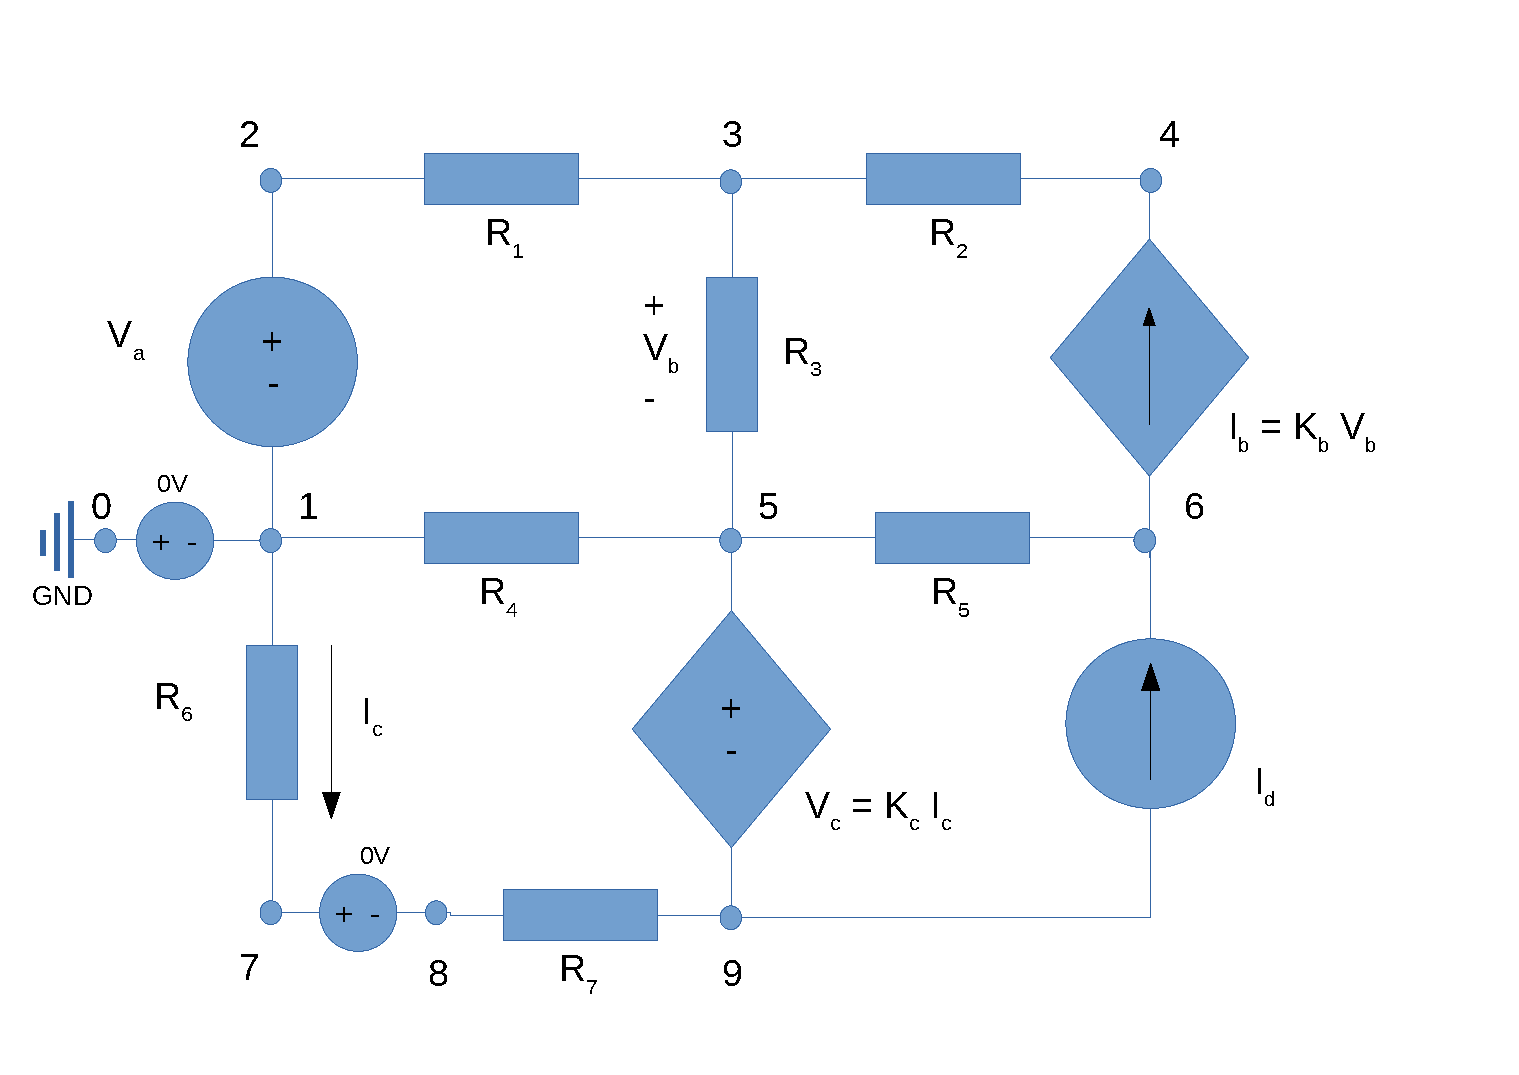
\includegraphics[width=0.8\linewidth]{circuit_sim.pdf}
\caption{Modified circuit for Ngspice simulation; numbers represent nodes.}
\label{fig:circuit_sim}
\end{figure}

\newpage

To properly analyse this circuit using Ngspice, it was convenient to slightly modify it. By defining the Ground voltage reference, we added a 0V voltage source between nodes 0 and 1, as shown in \ref{fig:circuit_sim}. To correctly define Vc, which is a CCVS that therefore requires a voltage source through which the controlling current flows, we had to add to the circuit another 0V voltage source. Because we knew that current Ic (which controlled Vc) flew through R6, we decided to add the aforementioned voltage source between resistors R6 and R7.
Despite being necessary to the sucess of the simulation, these modifications create an equivalent circuit. This means that these additions do not compromise the analysis of the original circuit in any way.

Table \ref{tab:op} shows the simulated operating point results for the circuit
under analysis. Compared to the theoretical analysis results, one notices that: the values obtained by simulating the circuit are identical in absolute value when compared to the theoretical predictions; the only notable difference is that while some theoretical values of current are negative, the ones obtained by the simulation are positive. This is a result of the arbitrary decision of the direction of the currents in each mesh. A negative value means that the actual direction of the current is the opposite of the one chosen.

\begin{table}[hp]
\centering
  \begin{tabular}{|l|r|}
    \hline    
    {\bf Name} & {\bf Value [A or V]} \\ \hline
   @cb[i] & 0.000000e+00\\ \hline
@ce[i] & 0.000000e+00\\ \hline
@q1[ib] & 7.022567e-05\\ \hline
@q1[ic] & 1.404513e-02\\ \hline
@q1[ie] & -1.41154e-02\\ \hline
@q1[is] & 5.765392e-12\\ \hline
@rc[i] & 1.411536e-02\\ \hline
@re[i] & 1.411536e-02\\ \hline
@rf[i] & 7.022567e-05\\ \hline
@rs[i] & 0.000000e+00\\ \hline
v(1) & 0.000000e+00\\ \hline
v(2) & 0.000000e+00\\ \hline
base & 2.254108e+00\\ \hline
coll & 5.765392e+00\\ \hline
emit & 1.411536e+00\\ \hline
vcc & 1.000000e+01\\ \hline

 \end{tabular}
  \caption{Operating point. A variable preceded by @ is of type current and expressed in Ampere; other variables are of type voltage and expressed in Volt.} 
  \label{tab:op}
\end{table}





